
\section{Introduction}

A regex is a syntax used to define a pattern
that can then be matched against strings for
validation or data extraction.

To represent a regex $r$, one usually uses its
non-deterministic finite automaton (NFA)
\cite{thompson_programming_1968}, computed in $O(|r|)$
time complexity and which has $O(|r|)$ nodes.

\input{chapters/1-introduction/sample-nfas.tex}

In the context of a regex, a capturing group $(X)$ can be used for the
extraction of subpatterns in a string. For example, one could use the regex
$(\textbackslash d \{ 4 \})-(\textbackslash d \{ 2 \})-(\textbackslash d \{ 2 \})$
to extract the year, month and day from a date in YYYY-MM-DD format.

To account for this, some special nodes are added to the NFA that
perform an action when visited, such as tracking the current string
position. For example, the node $\#1:entry$ keeps track of the index
of the string at which it entered the group $1$.

\begin{center}
    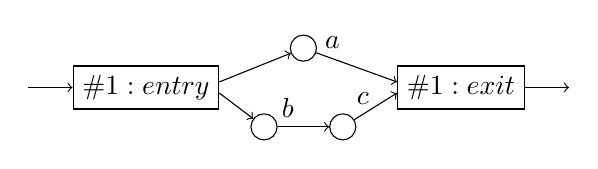
\begin{tikzpicture}
        \node[draw] (entry) at (-0.5, 0) {$\#1:entry$};
        \node[draw, circle] (up_a) at (1.5, 0.5) {};
        \node[draw, circle] (dw_b) at (1, -0.5) {};
        \node[draw, circle] (dw_c) at (2, -0.5) {};
        \node[draw] (exit) at (3.5, 0) {$\#1:exit$};

        \draw[->] ([xshift=-16]entry.west) -- (entry);
        \draw[->] ([yshift= 2pt]entry.east) -- (up_a);
        \draw[->] ([yshift=-2pt]entry.east) -- (dw_b);
        \draw[->] (dw_b) -- node[pos=0.2, above] (b) {$b$} (dw_c);
        \draw[->] (up_a) -- node[pos=0.2, above] (a) {$a$} ([yshift= 2pt]exit.west);
        \draw[->] (dw_c) -- node[pos=0.2, above] (c) {$c$} ([yshift=-2pt]exit.west);
        \draw[->] (exit) -- ([xshift=16]exit.east);
    \end{tikzpicture} \\ \vspace{0.3ex}
    \textit{NFA construction for $(a|bc)$}
\end{center}

\subsection{PikeVM Algorithm}

% TODO write some introduction about NFA, thread, priority, bytecode
% TODO also explain why there exists O(r) threads
